\documentclass{article}
\textheight 23.5cm \textwidth 15.8cm
%\leftskip -1cm
\topmargin -1.5cm \oddsidemargin 0.3cm \evensidemargin -0.3cm
%\documentclass[final]{siamltex}

\usepackage{verbatim}
\usepackage{fancyhdr}
\usepackage{amssymb,ctex}
\usepackage{mathrsfs}
\usepackage{latexsym,amsmath,amssymb,amsfonts,epsfig,graphicx,cite,psfrag}
\usepackage{eepic,color,colordvi,amscd}
\usepackage{enumerate}



\title{Numerical Analysis Homework1}
\author{Zhang Jiyao,PB20000204}

\begin{document}
	\maketitle
	
	\section{Introduction}
	
	计算汉明级数[Hamming(1962)]
	$$\varphi(x)=\sum_{k=1}^{\infty}\frac{1}{k(k+x)}$$
	其中$x$的取值为$x=0.0,0.1,0.2,...1.0,10.0,20.0,..300.0$共41个值,要求误差小于$10^{-6}$,并给出相应的$k$的取值上界。
	
	\section{Method}
	
	为了计算这个级数,我认为采取直接累加的方法是不可取的。不仅可能损失精度,还有可能导致复杂度过高。因此我打算参考计算多项式时的思路,改进这个算法。
	
	我们首先考虑$x$为整数的情况。当$x=1$时,我们通过裂项可以直接算出$\varphi(1)=1$.那么接下来都考虑$x$为整数的情况。对此,我们有
	
	$$\varphi(x)=\sum_{k=1}^{\infty}(\frac{1}{k}-\frac{1}{k+x})\frac{1}{x}$$
	$$\varphi(x+1)=\frac{1}{x+1}\sum_{k=1}^{\infty}(\frac{1}{k}-\frac{1}{k+x+1})$$
	$$(x+1)\varphi(x+1)-x\varphi(x)=\sum_{k=1}^{\infty}(\frac{1}{k+x}-\frac{1}{k+x+1})=-\frac{1}{x+1}$$
	
	$$\varphi(x+1)=\frac{x\varphi(x)+\frac{1}{x+1}}{(x+1)}$$
	那么在$x$为整数的情况下,我们就能通过递推式和初值$\varphi(1)=1$得出所有的$\varphi(x)$,$x$为整数。
	
	同样的,对$x$为小数的情况,我们也可以做类似的分析。
	
	$$\varphi(x)=\sum_{k=1}^{\infty}\frac{1}{k(k+x)},\varphi(1)=\sum_{k=1}^{\infty}\frac{1}{k(k+1)}$$
	
	$$f(x)=\varphi(x)-\varphi(1)=\sum_{k=1}^{\infty}\frac{1-x}{k(k+1)(k+x)}$$
	
	$$F(x)=\frac{f(x)}{1-x}=\sum_{k=1}^{\infty}\frac{1}{k(k+1)(k+x)}$$
	
	$$g(x)=F(x)-F(2)=\sum_{k=1}^{\infty}\frac{2-x}{k(k+1)(k+2)(k+x)}$$
	
	$$\varphi(x)=[g(x)+F(2)](1-x)+\varphi(1)$$
	
	那么只需要注意到$F(2)=0.25$,$\varphi(1)=1$,代入计算即可。
	
	为了求对应的$k$的取值上界,我们就把之前求得的$\varphi(x)$当成精确值,然后从第一项开始求和,直到做差小于$10^{-6}$即可.具体的细节我们在后面的讨论会说到。
	
	\section{Results}
	
  
	
	\begin{figure}[htb]
		\begin{center}
			
			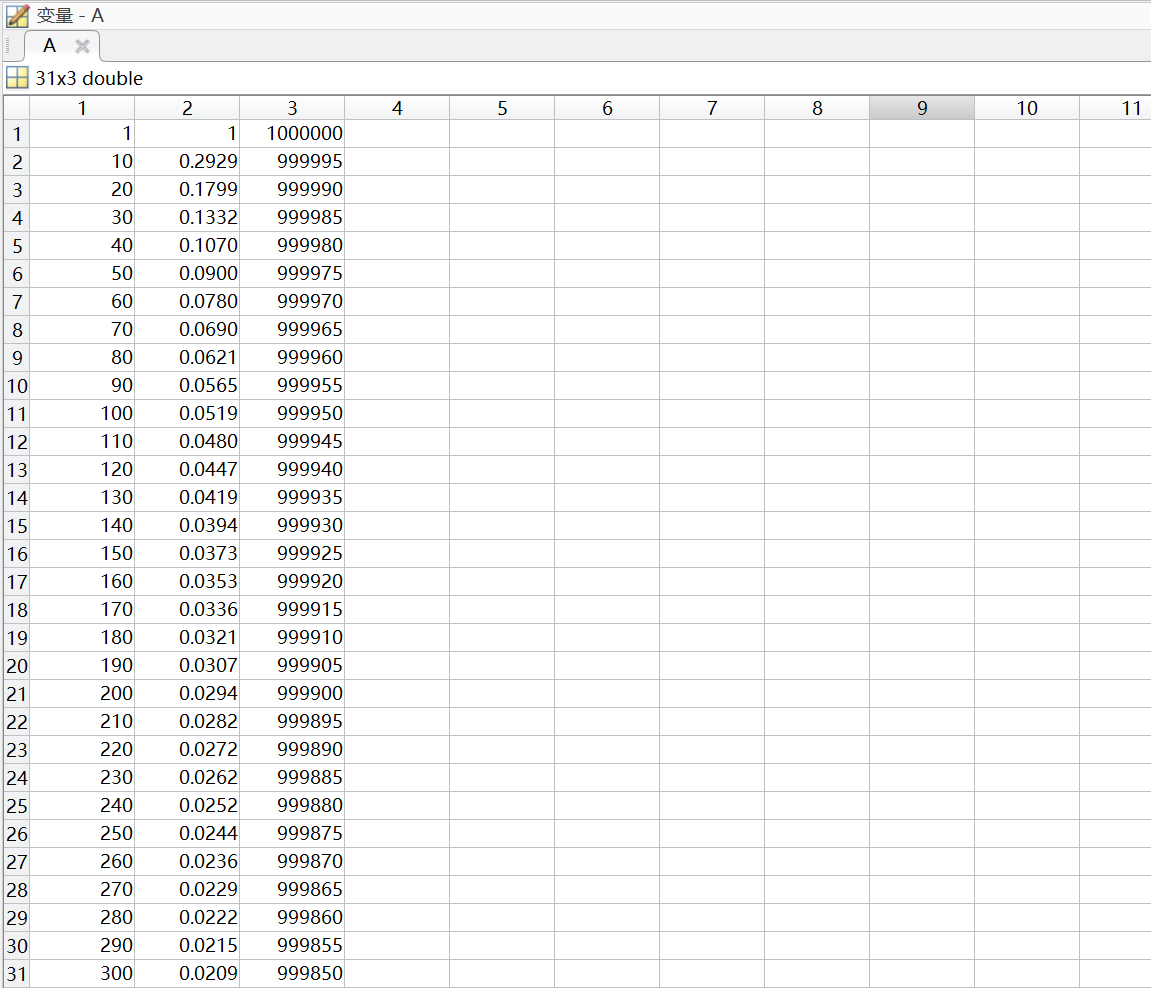
\includegraphics[width=12cm,height=13cm]{int1}
		
			\caption{当$x$为整数时的运行结果} \label{figure.label}
		\end{center}
	\end{figure}


	\begin{figure}[t]
	 \begin{center}
		
		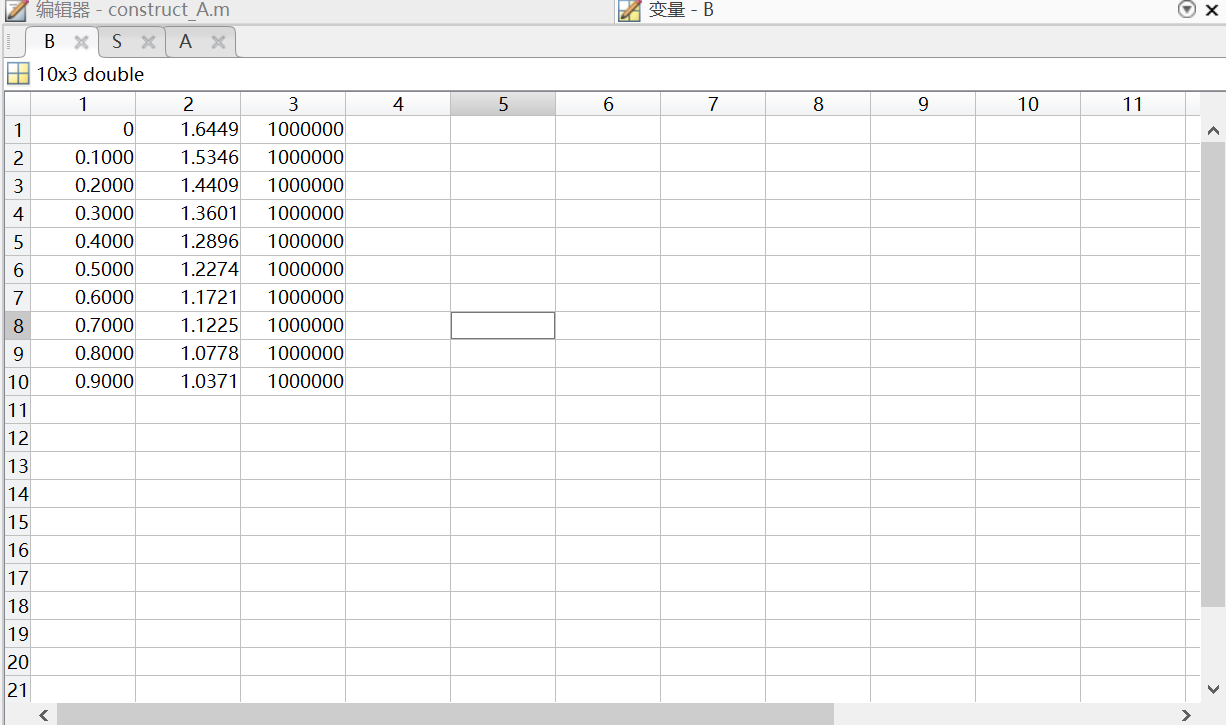
\includegraphics[width=12cm,height=12cm]{float}
		
		\caption{当$x$为小数时的运行结果} \label{figure.label}
	\end{center}
\end{figure}

\section{Discussion}

本次实验我是用MATLAB进行编程。

我一共编写了3个程序,一个是函数文件,用于计算递推的关系式。另外两个一个是$x$为整数的情况,一个是$x$为小数的情况.

在之前讨论$x$为小数的过程中,我们在最终计算求和时肯定只能取一个较大的$k$来计算。因为对余项我们有估计
$$\sum_{i=k}^{\infty}\frac{1}{i(i+x)} \leq \int_{k}^{\infty}\frac{1}{x^2}dx$$
因此只需要考虑$k$的阶数即可。因为题目要求了误差控制在$10^{-6}$次方以内,那么我们取一个$k=10^6$即可。此时$k^2$的阶数在$10^{12}$左右,在求$k$的上界过程中无影响.

得到的结果也是十分漂亮,在$x$为小数时求得的$k$全是$10^7$,但这个可能是由于设计的算法精度不够导致的。在$x$为整数时我们求得的为精确值,此时求得的$k$呈现出一个等差数列的规律。

\appendix
\section{Computer Code}

\small \hrule \verbatiminput{code.c} \hrule

$induction.m$

function y=induction(phi,x)

y=(x*phi+1/(x+1))/(x+1);

end

$construct_A.m$

A=zeros(31,3);

phi=zeros(1,301);

S=zeros(1,301);

K=zeros(1,31);

A(1,1)=1;

A(1,2)=1;

i=1;

j=1;

t=1;

phi(1)=1;

S(1)=1;

for i=2:300

phi(i)=induction(phi(i-1),i-1);

if i == 10*j

j=j+1;

A(j,1)=i;

A(j,2)=phi(i);

end	

end

s=1;

S(1)=phi(1);

while (S(1)>=1E-6)

S(1)=S(1)-1/(s*(s+1));

s=s+1;

end

A(1,3)=s-1;

for i=2:300

S(i)=phi(i);

s=1;

if i==10*t

while (S(i)>=1E-6)

S(i)=S(i)-1/(s*(s+i));

s=s+1;

end

A(t+1,3)=s-1;

t=t+1;

end

end

A

$construct_B.m$

phi=zeros(1,301);

S=zeros(1,10);

K=zeros(1,31);

B=zeros(10,3);

B(1,1)=0;

B(1,2)=pi*pi/6;

for x = 1 : 1 : 9

sum = 0;

for k = 1:100000

sum = sum + 1/(k*(k+0.1*x)*(k+1)*(k+2));

end

B(x+1,1)= x*0.1 ;

B(x+1,2)=(sum*(2-0.1*x)+0.25)*(1-0.1*x)+1;

end

for i = 1:10

s=1;

S(i)=B(i,2);

while(S(i)>=1E-6)

S(i)=S(i)-1/(s*(s+0.1*(i-1)));

s=s+1;

end

B(i,3)=s-1;

end

B
	
	
\end{document}